\documentclass[12pt]{article}

\usepackage{hyperref} % for auto-linking table of contents
\usepackage{amsmath}
\usepackage[margin=1in]{geometry}
\usepackage{fancyvrb} % fancy verbatim
\usepackage{fancyhdr}
\usepackage{graphicx}
\usepackage{float}
\usepackage{tikz} % for \foreach
\usepackage{caption}
\usepackage{subcaption}

\usepackage{paralist}
\usepackage{listings}
\usepackage{color}

\definecolor{dkgreen}{rgb}{0,0.6,0}
\definecolor{gray}{rgb}{0.5,0.5,0.5}
\definecolor{mauve}{rgb}{0.58,0,0.82}

\lstset{frame=tb,
  language=Matlab,
  aboveskip=3mm,
  belowskip=3mm,
  showstringspaces=false,
  columns=flexible,
  basicstyle={\small\ttfamily},
  numbers=none,
  numberstyle=\tiny\color{gray},
  keywordstyle=\color{blue},
  commentstyle=\color{dkgreen},
  stringstyle=\color{mauve},
  breaklines=true,
  breakatwhitespace=true
  tabsize=3
}


\hypersetup{
    bookmarks=true,         % show bookmarks bar?
    unicode=false,          % non-Latin characters in Acrobat�s bookmarks
    pdftoolbar=true,        % show Acrobat�s toolbar?
    pdfmenubar=true,        % show Acrobat�s menu?
    pdffitwindow=false,     % window fit to page when opened
    pdfstartview={FitH},    % fits the width of the page to the window
    pdftitle={My title},    % title
    pdfauthor={Author},     % author
    pdfsubject={Subject},   % subject of the document
    pdfcreator={Creator},   % creator of the document
    pdfproducer={Producer}, % producer of the document
    pdfkeywords={keyword1} {key2} {key3}, % list of keywords
    pdfnewwindow=true,      % links in new PDF window
    colorlinks=true,       % false: boxed links; true: colored links
    linkcolor=blue,          % color of internal links (change box color with linkbordercolor)
    citecolor=green,        % color of links to bibliography
    filecolor=magenta,      % color of file links
    urlcolor=blue           % color of external links
}
\usepackage[ampersand]{easylist}



\pagestyle{fancy}
\lhead{Daniel McArdle}
\chead{Homework 3}
\rhead{CSE 573: Computer Vision}
\cfoot{\thepage}


\begin{document}

\title{Homework 2: Segmentation}
\author{Daniel McArdle\\
CSE 573: Computer Vision}
\date{November 22, 2014}
\maketitle  % without this line, the header would not be generated

% \tableofcontents

\section{Report}

\subsection{Technique for Matching Textureless Regions}

To match textureless regions in stereo images, I would try to use information
about the nearest regions that do have textures. By finding the average
disparity of the closest textured regions, and by assuming uniform motion, we
could compute a best guess for the disparity of the textureless region.

The ``Reindeer" image is likely the one with the largest textureless region.
Unsurprisingly, this area of the disparity map is quite inaccurate.  When the
block-matching algorithm encounters a textureless region, any block matches any
other block from that region, causing inacurrate calculated disparities.

\subsection{MSE vs Window Size}

\subsection{MATLAB Optimizations}

The problems of block matching and the dynamic programming algorithm are quite
difficult to disentangle from looping control structures. For some operations
performed in the loops, however, I was able to use built-in MATLAB functions
for speed.

For example, in \texttt{BlockMatch.m}, rather than computing the SSD value with
loops, I simply created two submatrices \texttt{block1} and \texttt{block2}.
The SSD value of these blocks is \texttt{sum(sum( (block1 - block2) .\^ 2 ))}.

In \texttt{DynamicProg.m}, rather than computing the mean value of each arc
with a loop, I opted to use the built-in \texttt{mean} function.  

\subsection{Runtime Analysis}

\subsubsection{Block Matching}
With $m$ rows and $n$ columns, the block matching algorithm iterates over each
pixel, $O(mn)$ operations.  For each pixel, find the best column disparity,
meaning we are performing $O(mn^2)$ operations in total (although we can
restrict the range of columns searched, there is no asymptotic difference).
Then, for each disparity value tested, we compute the SSD, an operation that
takes $O(w^2)$ operations, where $w$ is the window size.

In total, the block matching algorithm is $O(mn^2w^2)$. When the number of
rows, $m$, is increased linearly, the runtime will increase linearly. When
either the number of columns, $n$, or the window size, $w$, is increased
linearly, the runtime will increase quadratically.

\subsubsection{Dynamic Programming}

The dynamic programming algorithm incorporates the textbook's scanline matching
algorithm. This means that we need to run the textbook's algorithm for each of
$m$ rows.  This gets us to $O(m)$.

For each row, we iterate over the edges from the first image and the edges from
the second image. In the pathological worst case, there would be $n$ edges in
each image, meaning the algorithm is up to $O(mn^2)$ running time.

For each pair of edges, we consider each of three inferior neighbors to this
pair.  Three is a constant factor, which can be ignored asymptotically.	For
each of these neighbors, we compute the ``Arc-Cost" of the corresponding two
arcs from the first and second images, which is an $O(1)$ operation, since the
length of an arc would be 1 if there are $n$ arcs total.

Ultimately, this makes the dynamic programming algorithm have a complexity of
$O(mn^2)$, but it is important to remember that the number of edges in a
scanline will likely be very small compared the number of columns.  So in
reality, the number of operations performed will be $O(mk^2)$ where $k$ is much
smaller than $n$.

\subsection{Literature Review}

For the literature review, I am choosing two papers that focus on accuracy and
efficiency, respectively. These are two features that my algorithm
implementations are sorely lacking. Interestingly, in the area of disparity
matching, there is usually a tradeoff between the two ~\cite{papertwo}.

\subsubsection{Paper 1: \textbf{Efficient Large Scale Stereo Matching} (2010)}
The main idea of \textbf{Efficient Large Scale Stereo Matching} is that many
computed stereo correspondences will be ambiguous, but some of them can be
``robustly matched." These ``support points" are then used to improve the
quality of the ambiguous correspondences.

This approach already has a major difference from our block matching algorithm.
Our block matching algorithm naievely chooses the disparity that causes a small
window of pixels to match best. This is naive because occlusion may cause a
window to be impossible to match. This can produce wildly-inaccurate disparity
values, which would not have occurred had we used support points. 

The algorithm outlined in the paper also takes multiple measures to preserve
consistency.  Similar to the block matching consistency check, they require
that correspondences match left-to-right and right-to-left.  They go one step
further, though, and ``eliminate all points whose ratio beween the best and
second best match exceeds a fixed threshold". In other words, they will not
accept possibly-ambiguous disparities.

The algorithm also makes use of a Probabilistic Generative Model that uses
support points to actually perform the stereo matching.


\subsubsection{Paper 2: \textbf{On building an accurate stereo matching system on graphics hardware} (2011)}

This paper was intriguing to me because it presents an algorithm that runs on
the GPU. The abstract boasts that it achieves near-real-time performance and is
the top performer in the Middlebury benchmark at the time of publication,
achieving results in 0.1 seconds. 

The algorithm uses techniques developed in multiple papers. The key features
are Cost Initialization, Cost Aggregation, Scanline Optimization, Disparity
Refinement. The final feature is an efficient GPU implementation using CUDA. 

Our algorithm would not lend itself well to GPU implementation, as GPUs are
highly parallel and our algorithm relies on mutable state.


\section{Results}

% Load the results_display file
\subsection{Data}
\begin{figure}[h]    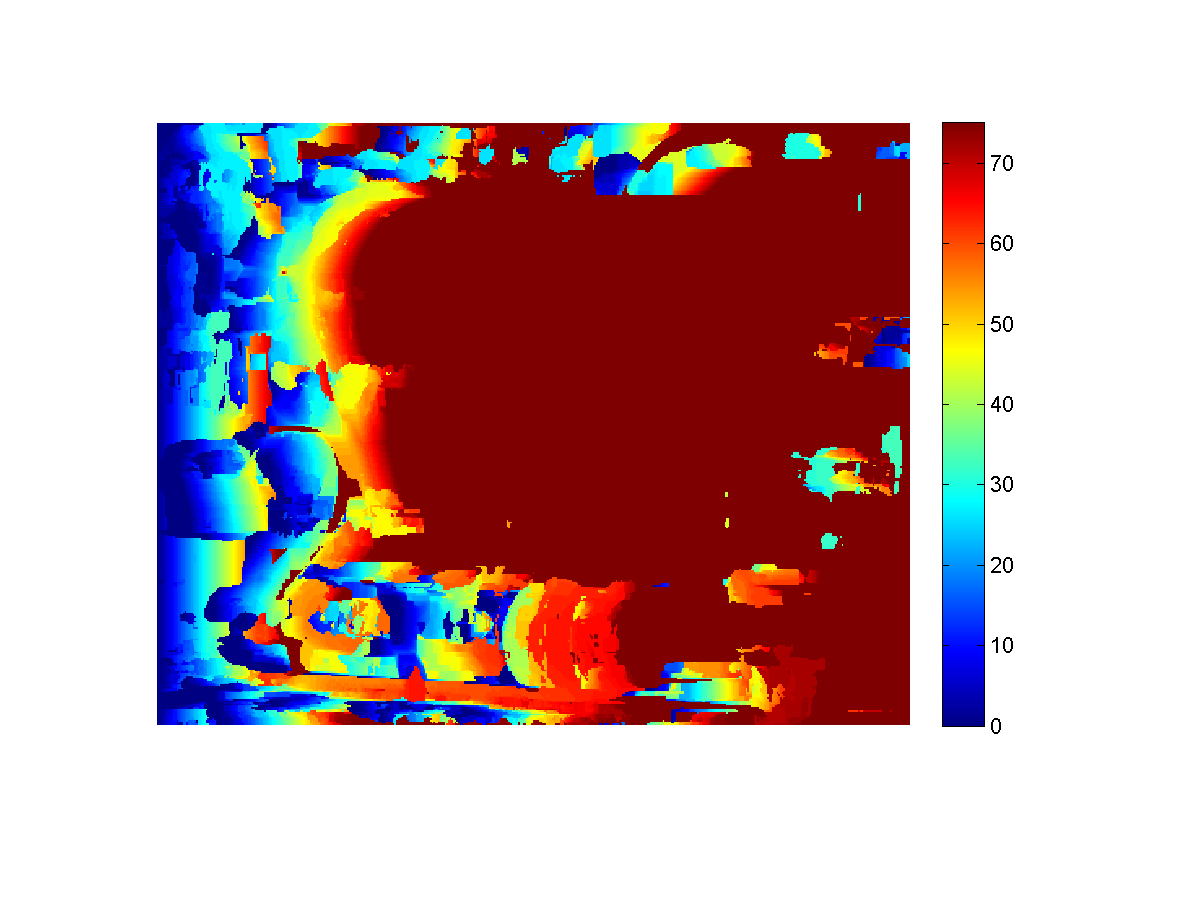
\includegraphics[scale=0.5]{output/Data/disp1.png}    \caption{output/Data/disp1.png}\end{figure}
\begin{figure}[h]    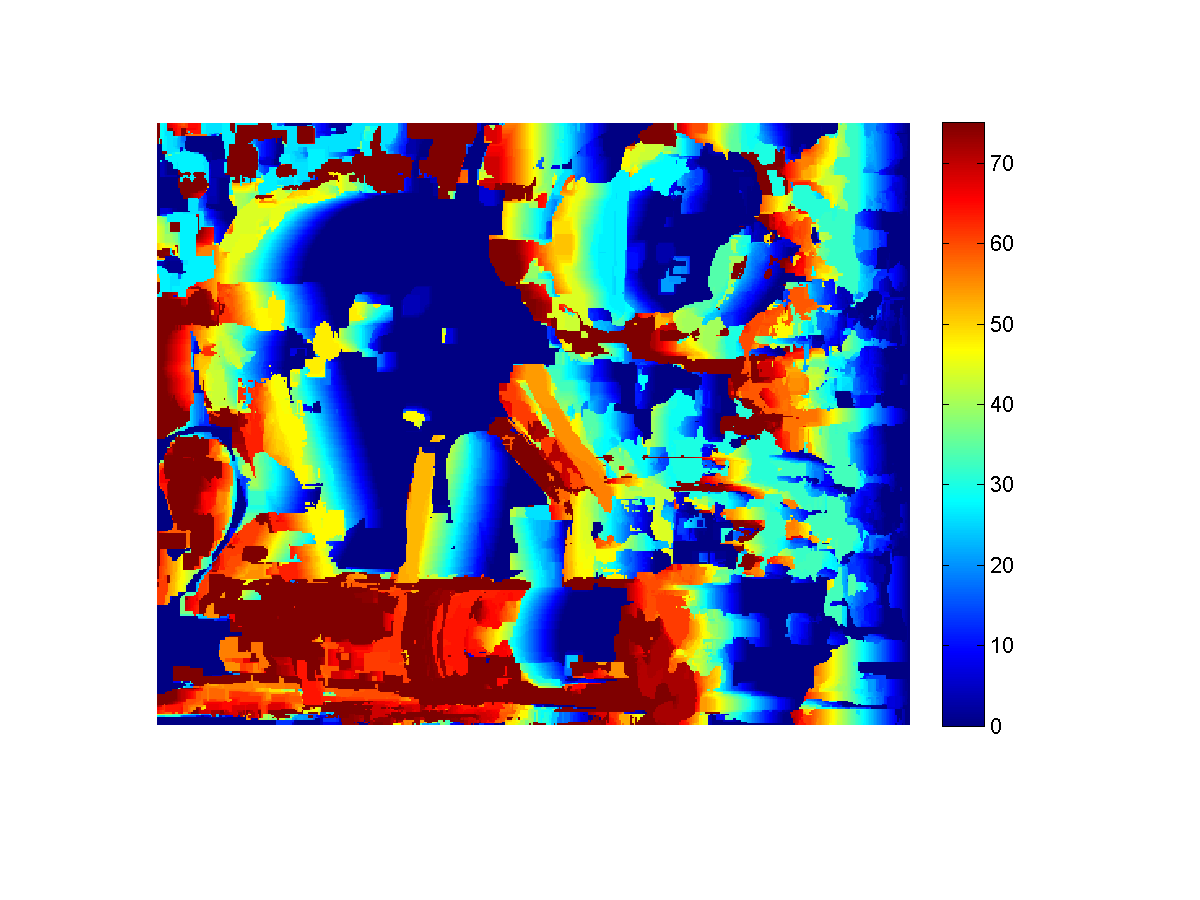
\includegraphics[scale=0.5]{output/Data/disp2.png}    \caption{output/Data/disp2.png}\end{figure}
\begin{figure}[h]    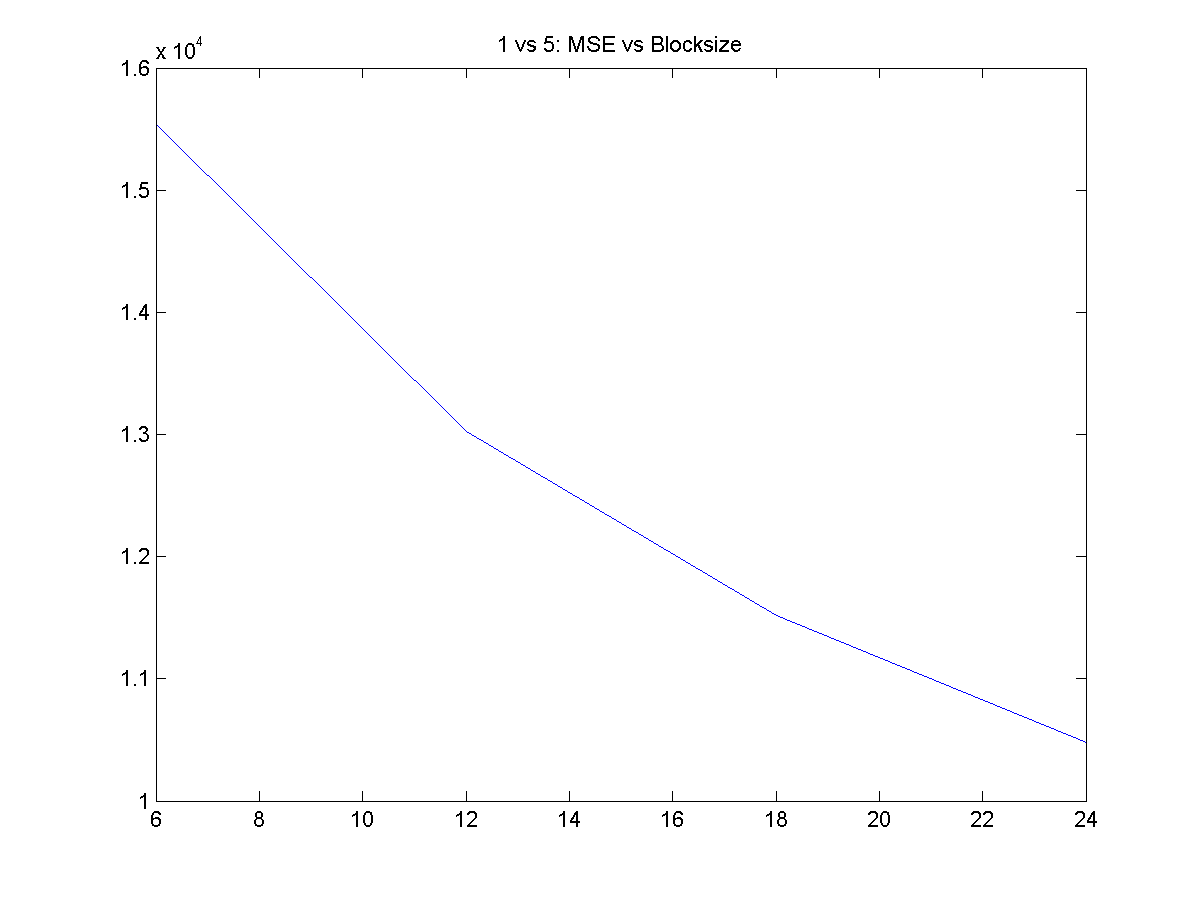
\includegraphics[scale=0.5]{output/Data/mse_vs_blocksize.png}    \caption{output/Data/mse\_vs\_blocksize.png}\end{figure}
\begin{figure}[h]    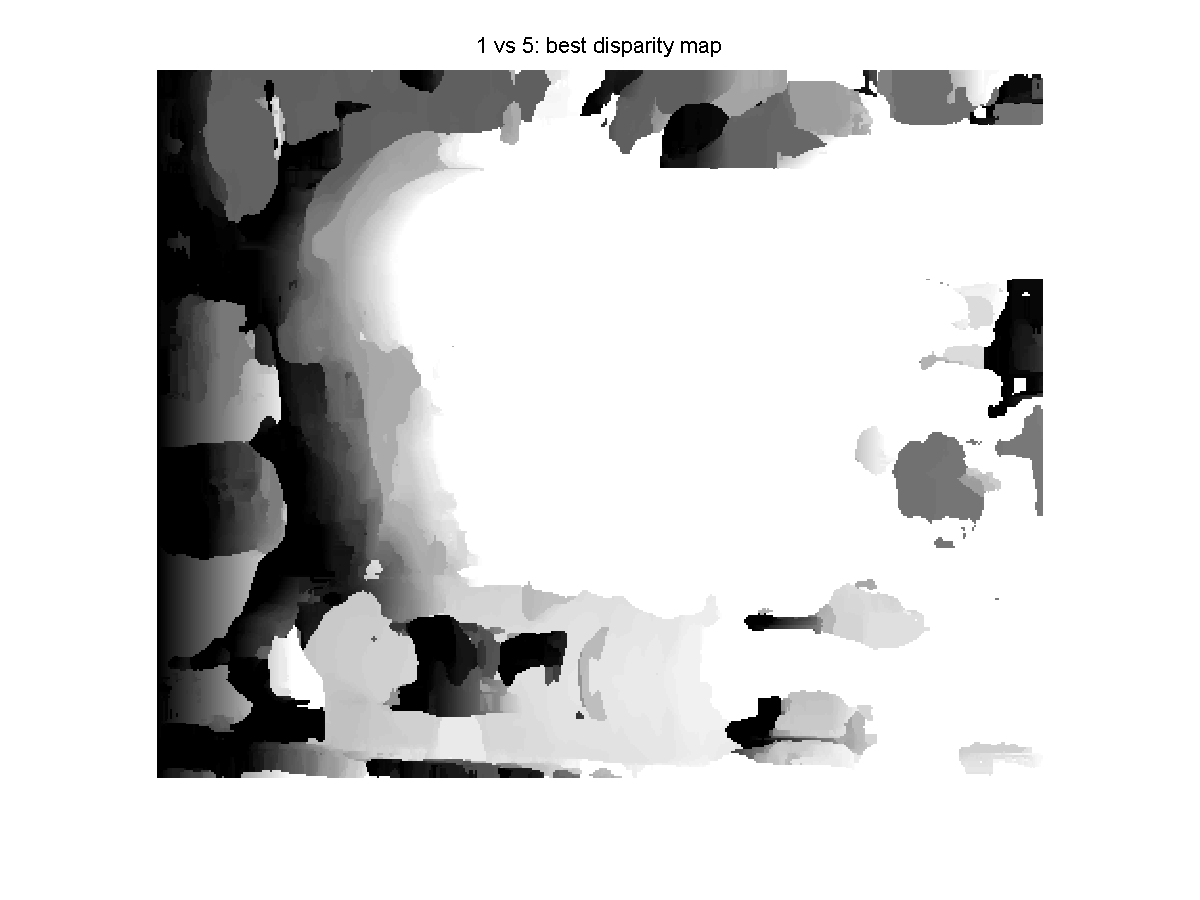
\includegraphics[scale=0.5]{output/Data/best_dispmap.png}    \caption{output/Data/best\_dispmap.png}\end{figure}
\begin{figure}[h]    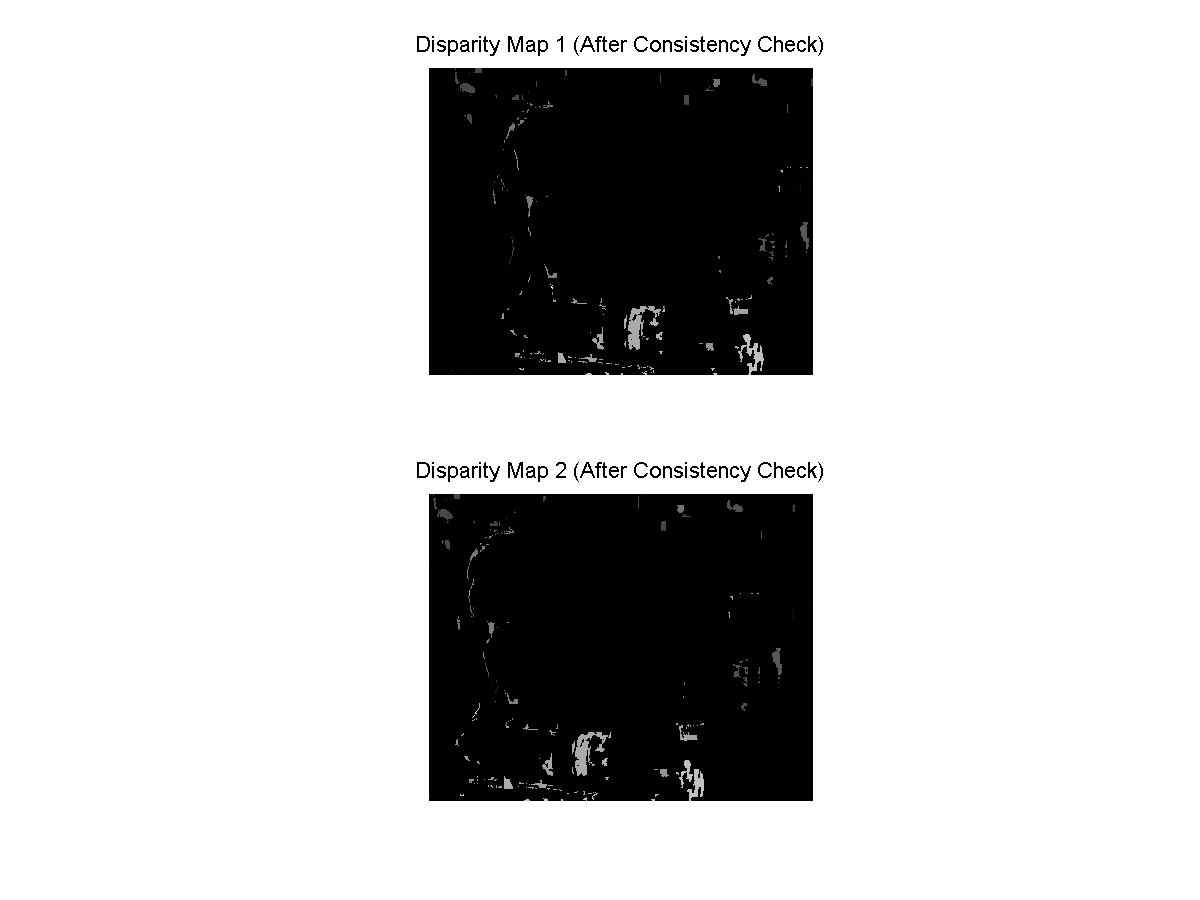
\includegraphics[scale=0.5]{output/Data/after_consistency_check.png}    \caption{output/Data/after\_consistency\_check.png}\end{figure}
\begin{figure}[h]    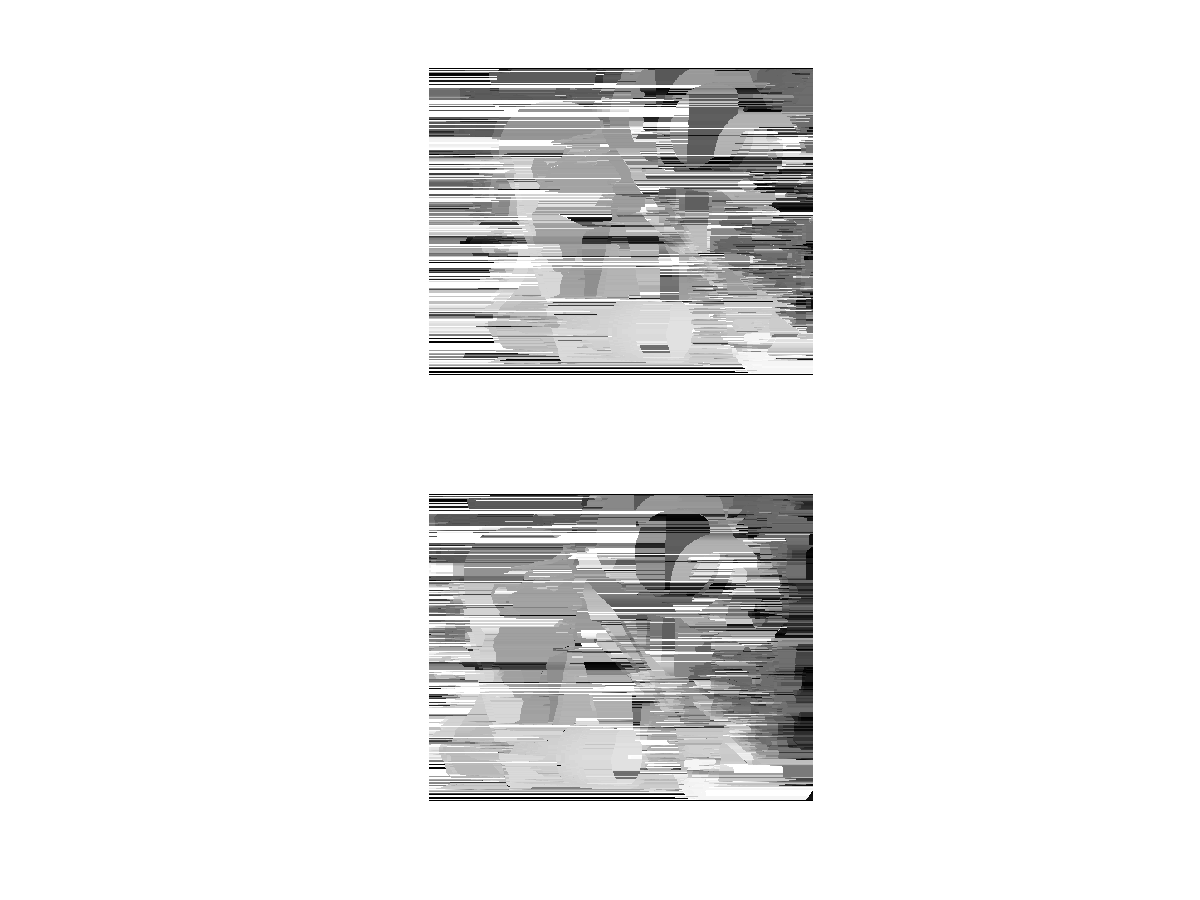
\includegraphics[scale=0.5]{output/Data/dynamic_prog.png}    \caption{output/Data/dynamic\_prog.png}\end{figure}
\subsection{Books}
\begin{figure}[h]    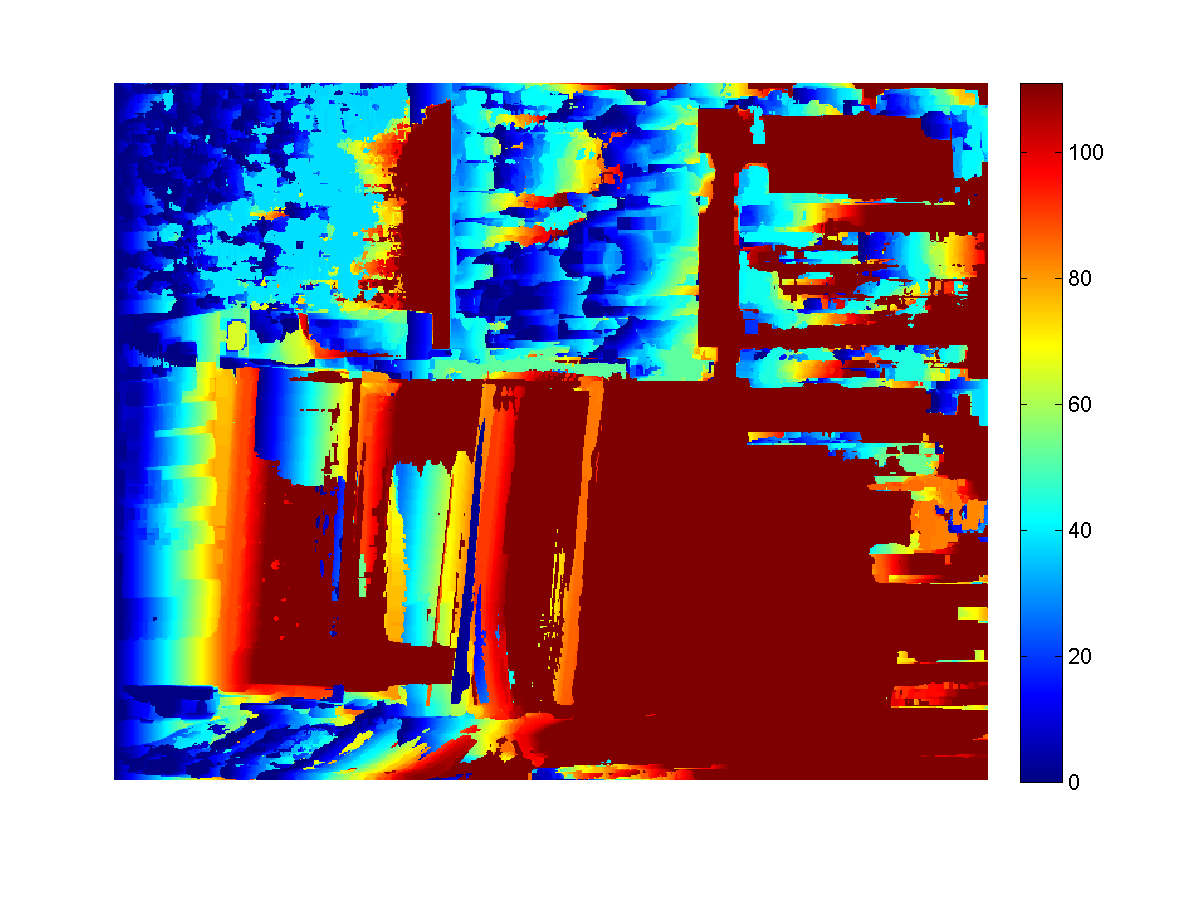
\includegraphics[scale=0.5]{output/Evaluation/Books/disp1.png}    \caption{output/Evaluation/Books/disp1.png}\end{figure}
\begin{figure}[h]    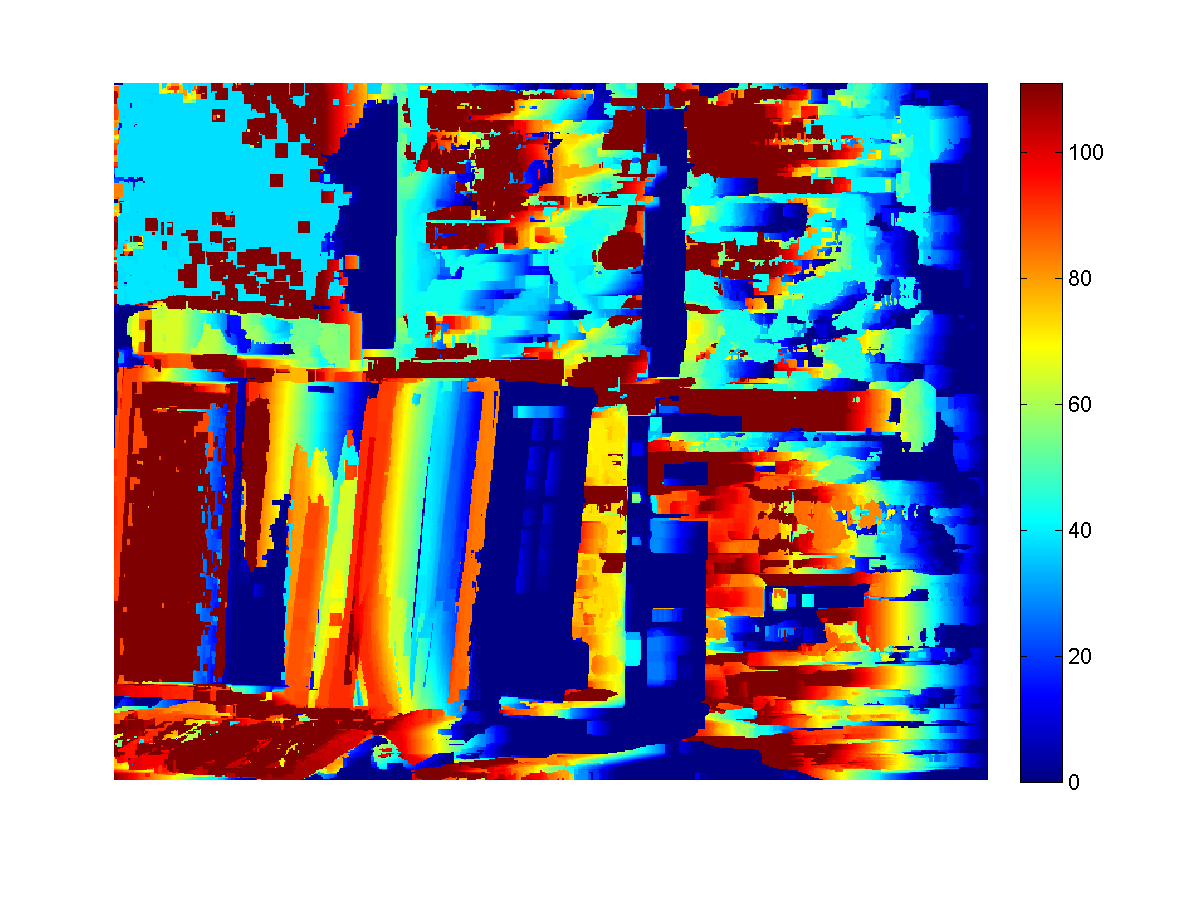
\includegraphics[scale=0.5]{output/Evaluation/Books/disp2.png}    \caption{output/Evaluation/Books/disp2.png}\end{figure}
\begin{figure}[h]    \includegraphics[scale=0.5]{output/Evaluation/Books/mse_vs_blocksize.png}    \caption{output/Evaluation/Books/mse\_vs\_blocksize.png}\end{figure}
\begin{figure}[h]    \includegraphics[scale=0.5]{output/Evaluation/Books/best_dispmap.png}    \caption{output/Evaluation/Books/best\_dispmap.png}\end{figure}
\begin{figure}[h]    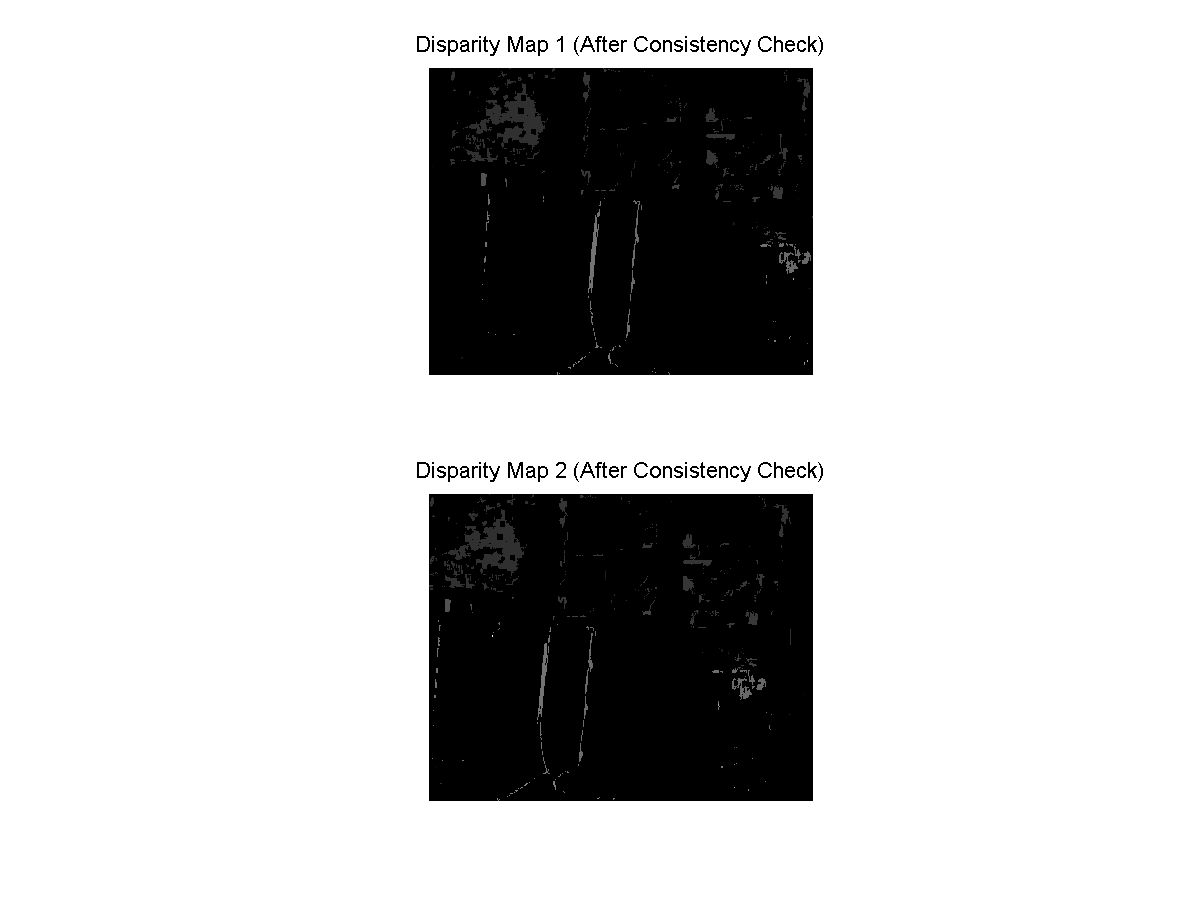
\includegraphics[scale=0.5]{output/Evaluation/Books/after_consistency_check.png}    \caption{output/Evaluation/Books/after\_consistency\_check.png}\end{figure}
\begin{figure}[h]    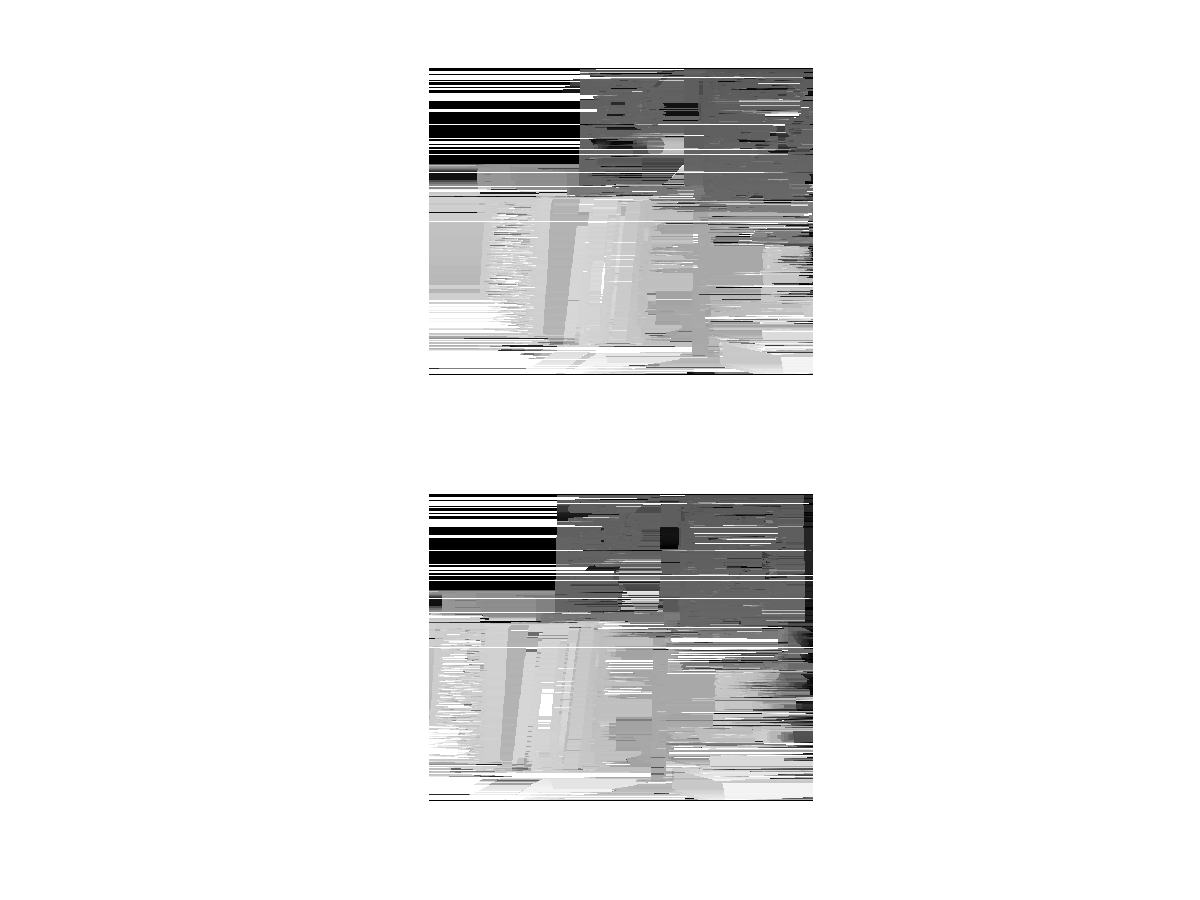
\includegraphics[scale=0.5]{output/Evaluation/Books/dynamic_prog.png}    \caption{output/Evaluation/Books/dynamic\_prog.png}\end{figure}
\subsection{Dolls}
\begin{figure}[h]    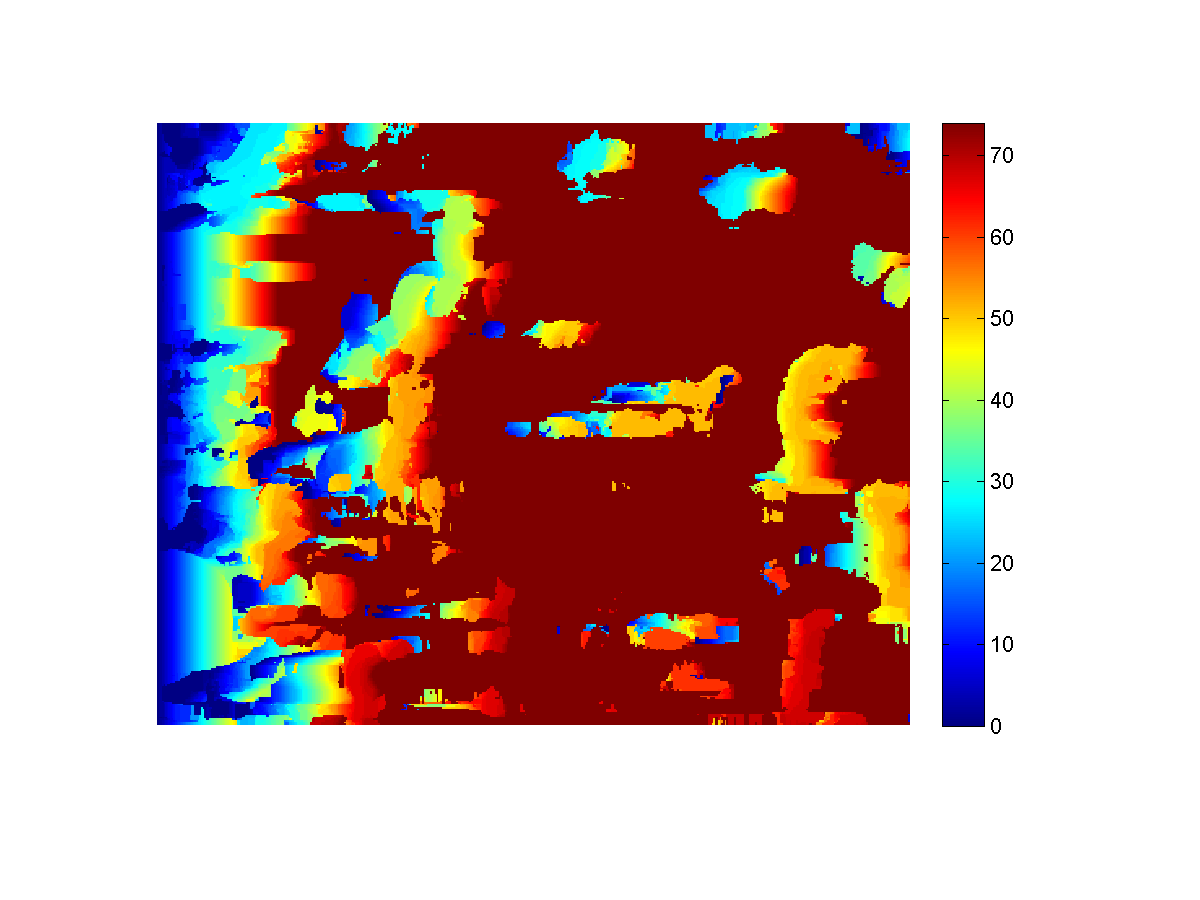
\includegraphics[scale=0.5]{output/Evaluation/Dolls/disp1.png}    \caption{output/Evaluation/Dolls/disp1.png}\end{figure}
\begin{figure}[h]    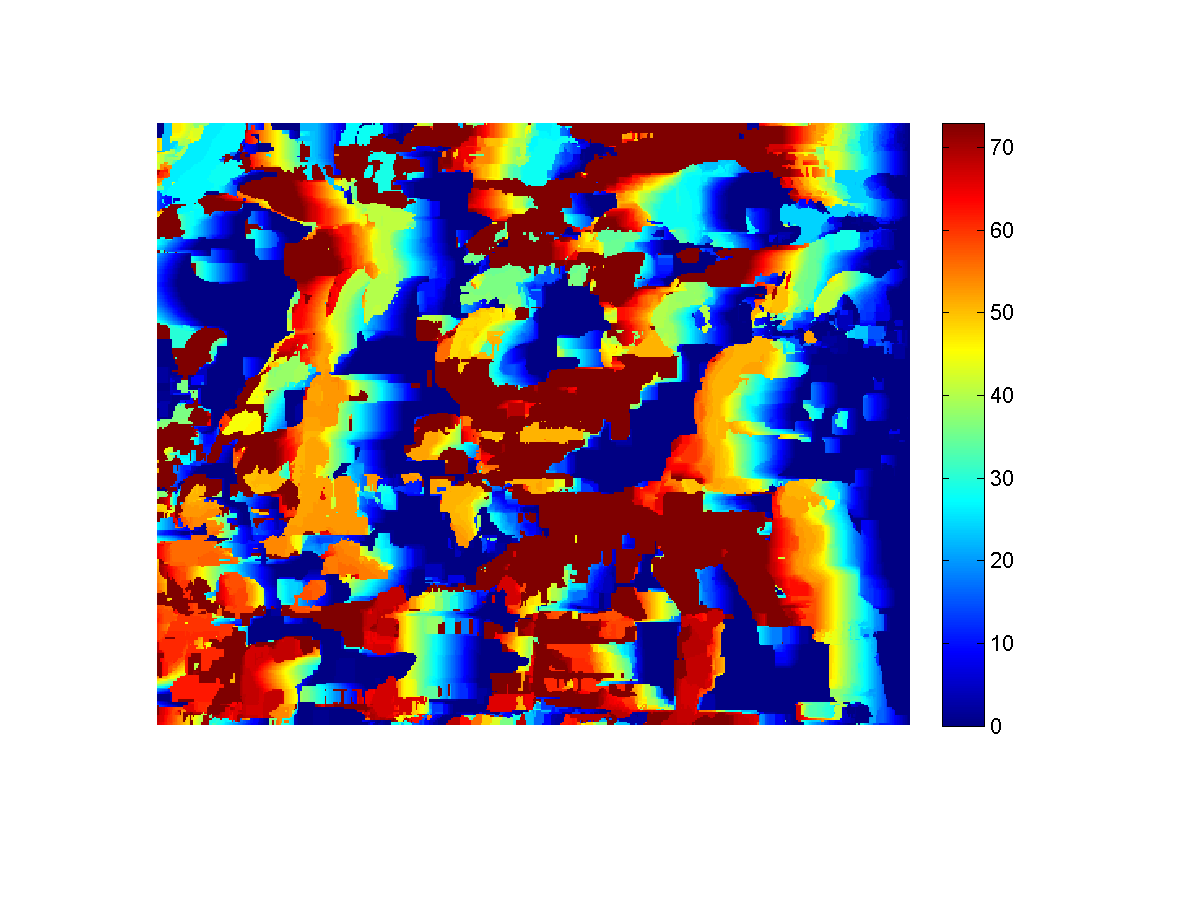
\includegraphics[scale=0.5]{output/Evaluation/Dolls/disp2.png}    \caption{output/Evaluation/Dolls/disp2.png}\end{figure}
\begin{figure}[h]    \includegraphics[scale=0.5]{output/Evaluation/Dolls/mse_vs_blocksize.png}    \caption{output/Evaluation/Dolls/mse\_vs\_blocksize.png}\end{figure}
\begin{figure}[h]    \includegraphics[scale=0.5]{output/Evaluation/Dolls/best_dispmap.png}    \caption{output/Evaluation/Dolls/best\_dispmap.png}\end{figure}
\begin{figure}[h]    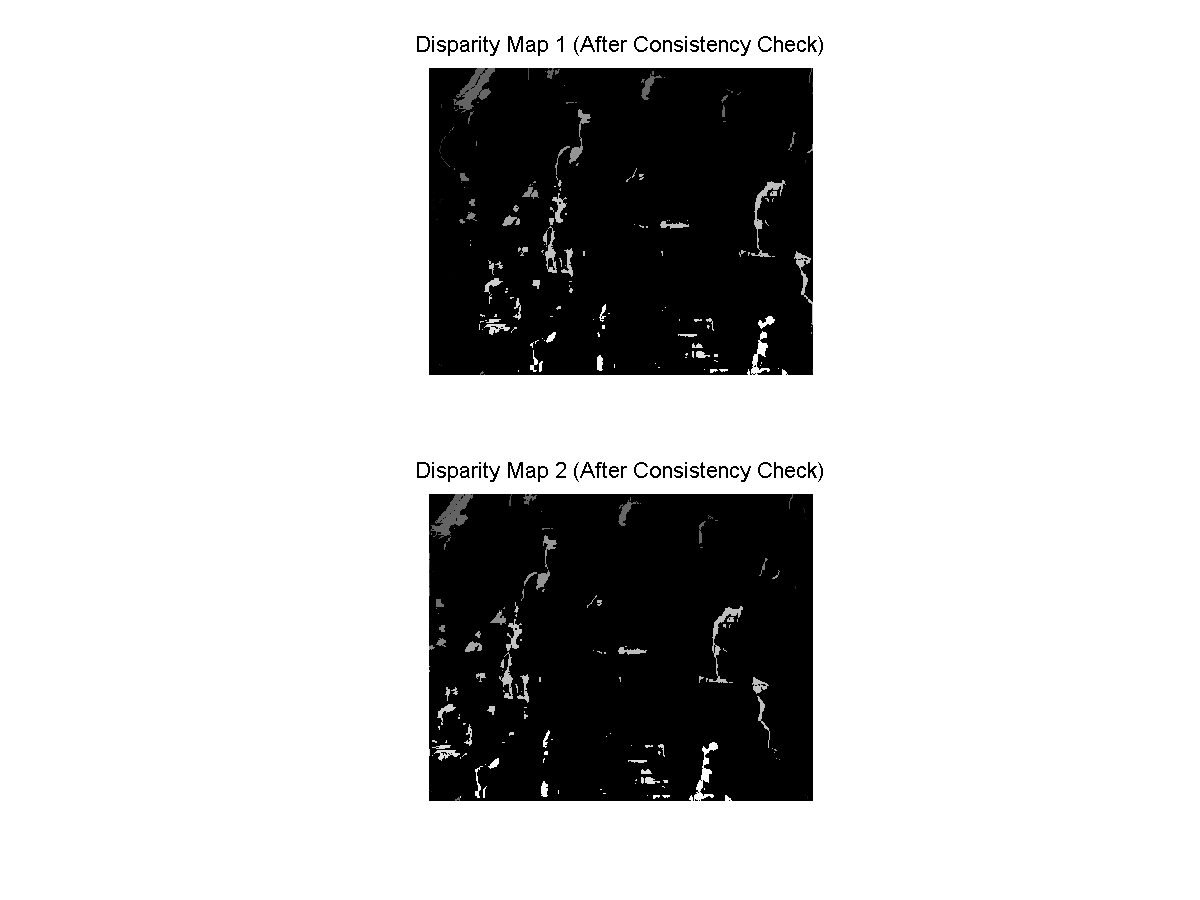
\includegraphics[scale=0.5]{output/Evaluation/Dolls/after_consistency_check.png}    \caption{output/Evaluation/Dolls/after\_consistency\_check.png}\end{figure}
\begin{figure}[h]    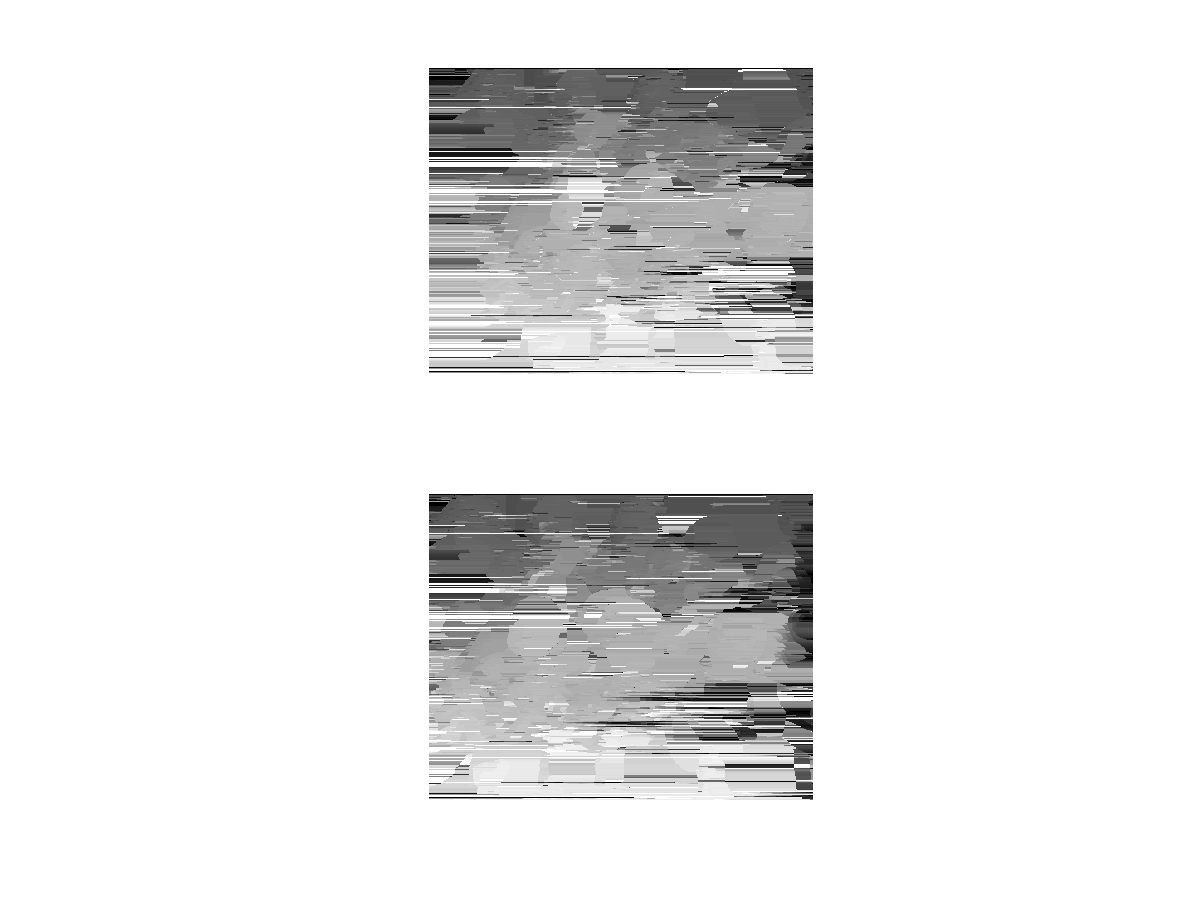
\includegraphics[scale=0.5]{output/Evaluation/Dolls/dynamic_prog.png}    \caption{output/Evaluation/Dolls/dynamic\_prog.png}\end{figure}
\subsection{Reindeer}
\begin{figure}[h]    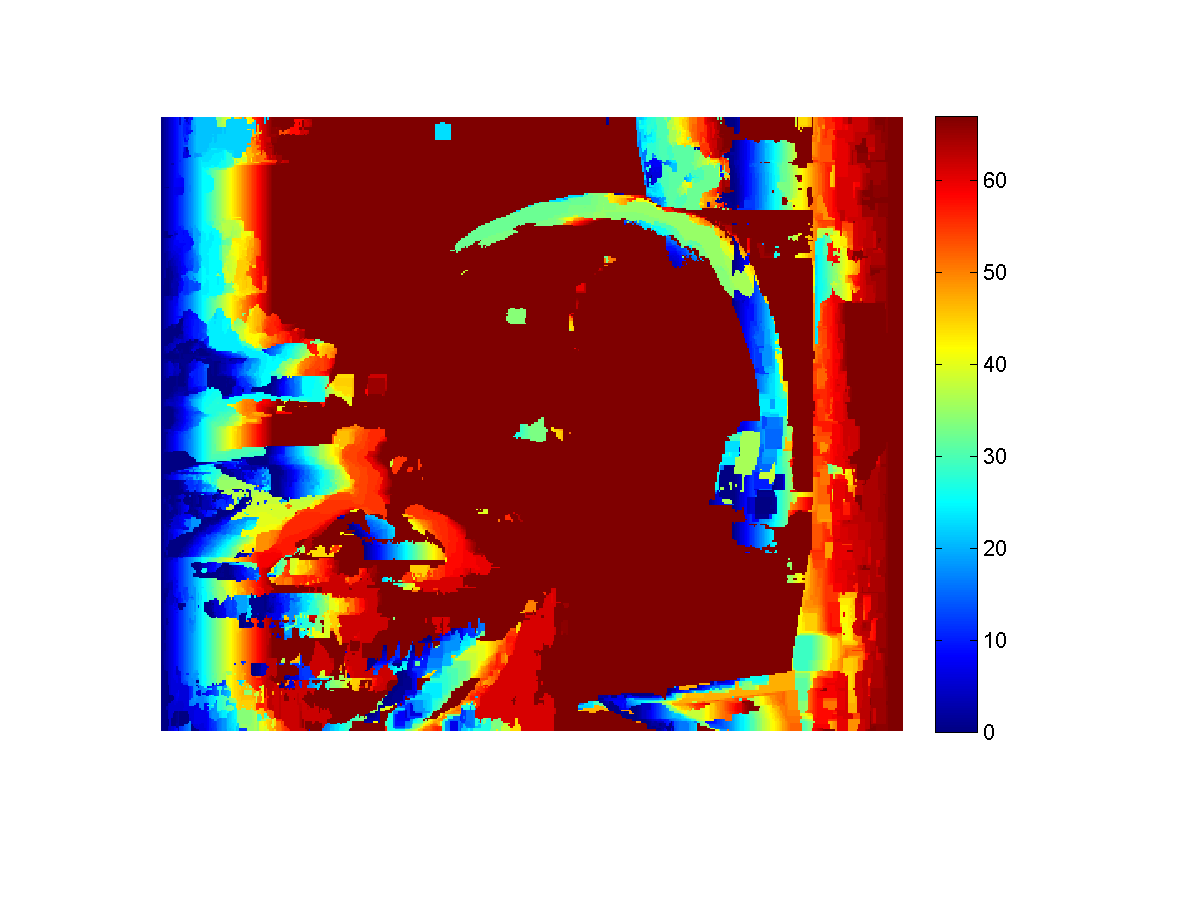
\includegraphics[scale=0.5]{output/Evaluation/Reindeer/disp1.png}    \caption{output/Evaluation/Reindeer/disp1.png}\end{figure}
\begin{figure}[h]    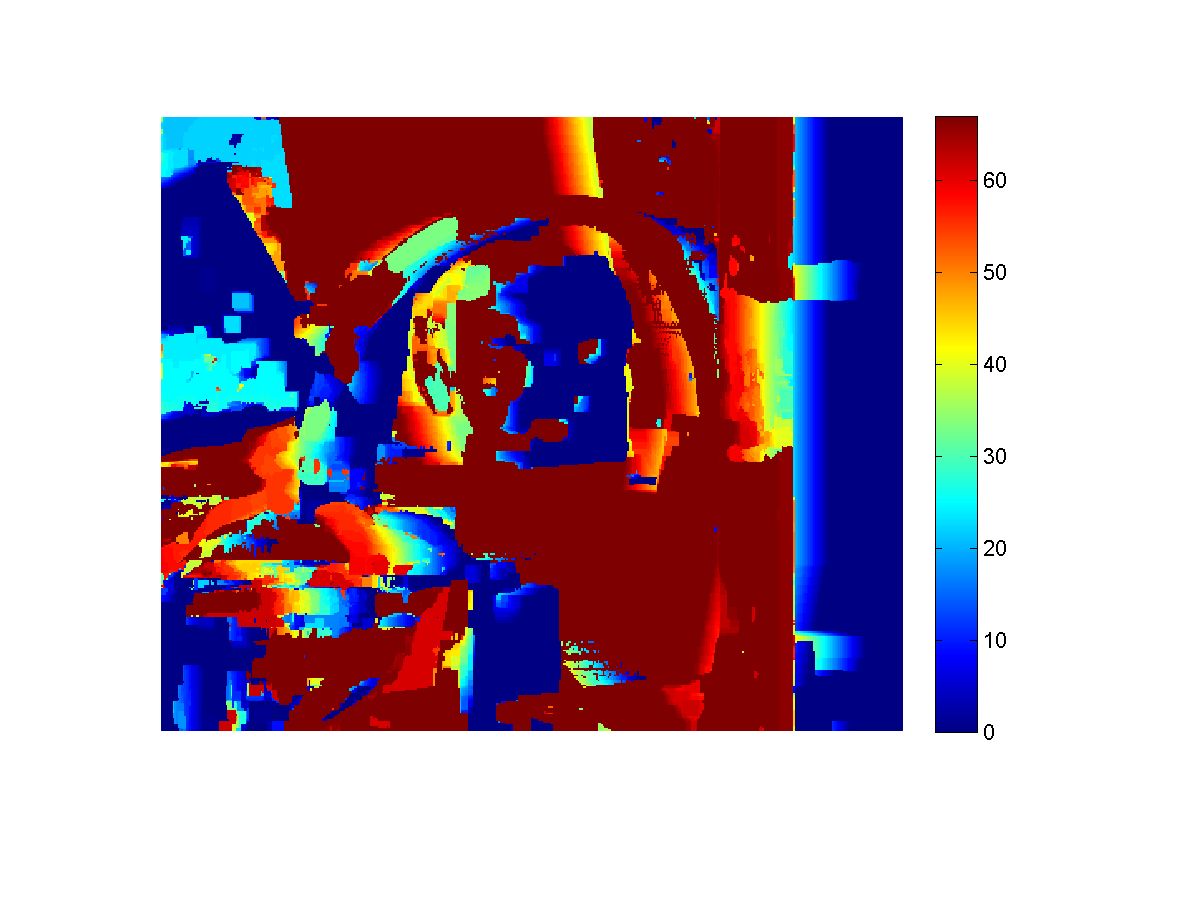
\includegraphics[scale=0.5]{output/Evaluation/Reindeer/disp2.png}    \caption{output/Evaluation/Reindeer/disp2.png}\end{figure}
\begin{figure}[h]    \includegraphics[scale=0.5]{output/Evaluation/Reindeer/mse_vs_blocksize.png}    \caption{output/Evaluation/Reindeer/mse\_vs\_blocksize.png}\end{figure}
\begin{figure}[h]    \includegraphics[scale=0.5]{output/Evaluation/Reindeer/best_dispmap.png}    \caption{output/Evaluation/Reindeer/best\_dispmap.png}\end{figure}
\begin{figure}[h]    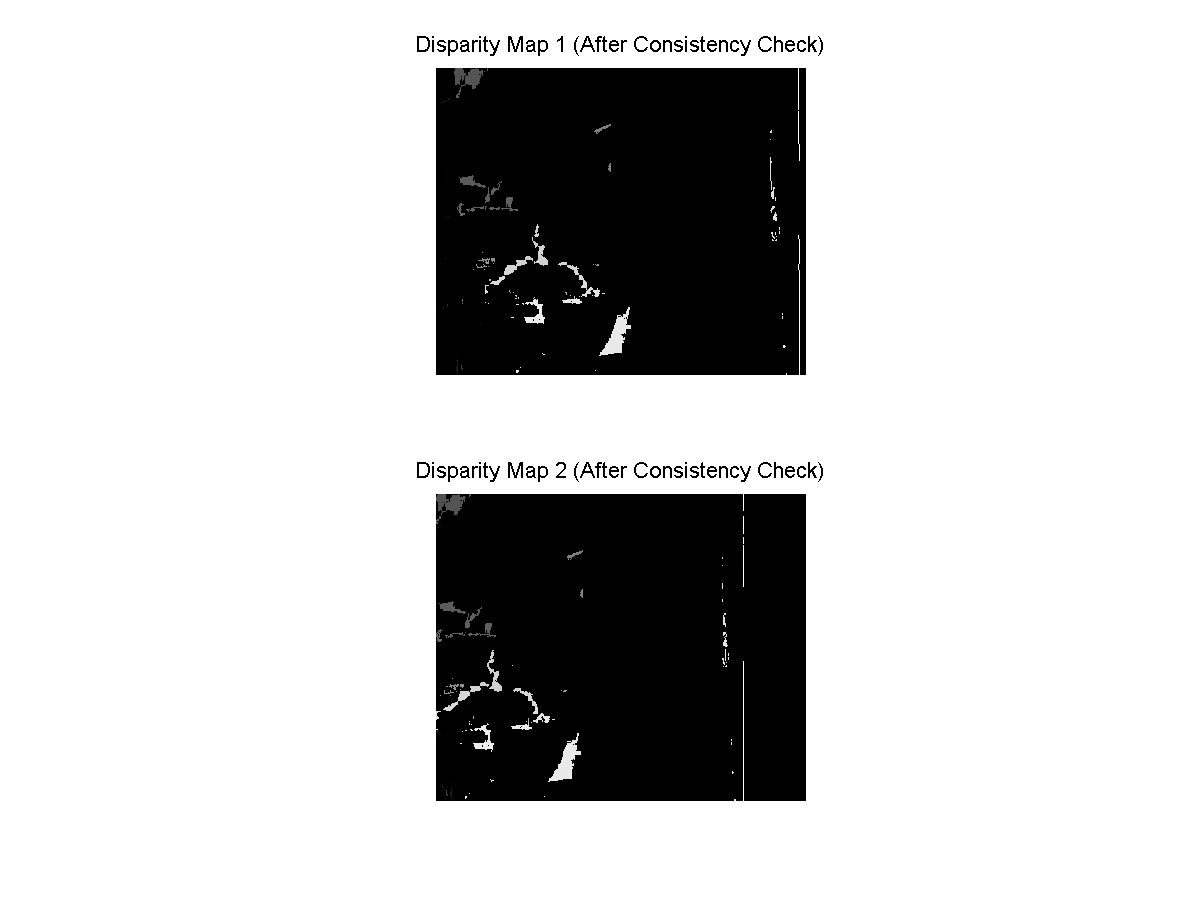
\includegraphics[scale=0.5]{output/Evaluation/Reindeer/after_consistency_check.png}    \caption{output/Evaluation/Reindeer/after\_consistency\_check.png}\end{figure}
\begin{figure}[h]    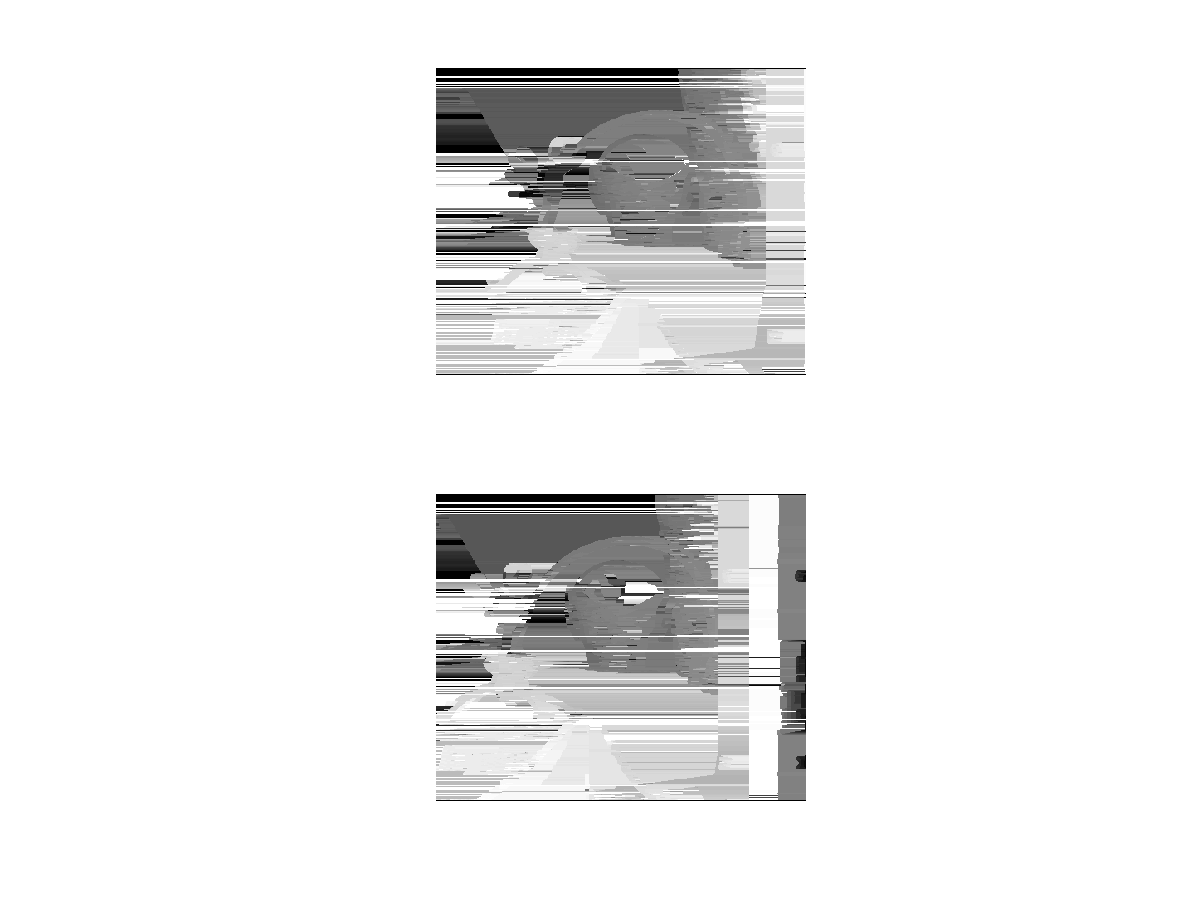
\includegraphics[scale=0.5]{output/Evaluation/Reindeer/dynamic_prog.png}    \caption{output/Evaluation/Reindeer/dynamic\_prog.png}\end{figure}


\bibliography{biblio}





\end{document}

